\documentclass{article}
\usepackage{tikz}
\usetikzlibrary{arrows,decorations.pathmorphing}

\begin{document}
\begin{center}
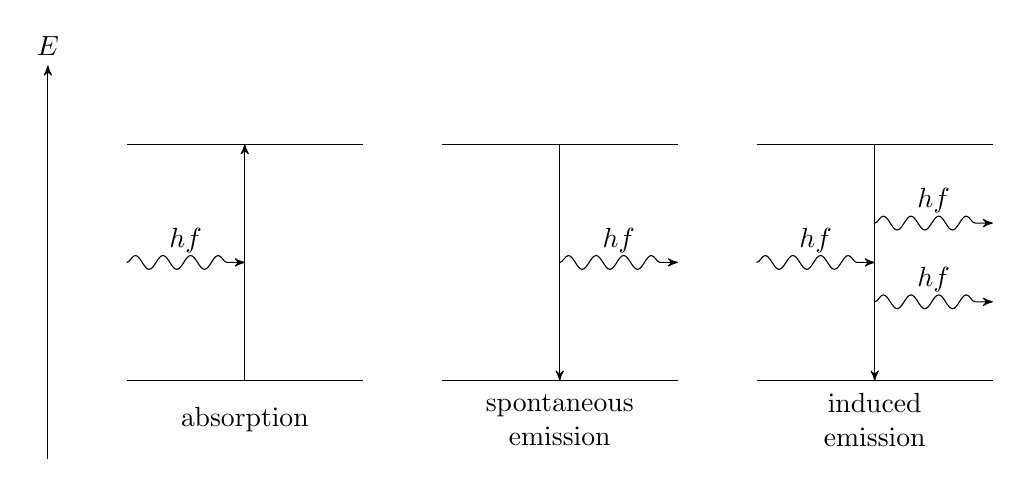
\begin{tikzpicture}[
  >=stealth',
  pos=.8,
  photon/.style={decorate,decoration={snake,post length=1mm}}
  ]
%\draw [ultra thin, lightgray] (0,0) grid (13,5);
\draw [->] (0,0) -- (0,5);
\node [above] at (0,5) {\(E\)};
\draw (1,1) -- (4,1);
\draw (5,1) -- (8,1);
\draw (9,1) -- (12,1);
\draw (1,4) -- (4,4);
\draw (5,4) -- (8,4);
\draw (9,4) -- (12,4);
\draw [<-] (2.5,4) -- (2.5,1);
\draw [->] (6.5,4) -- (6.5,1);
\draw [->] (10.5,4) -- (10.5,1);
\draw [->, photon](1,2.5) -- (2.5,2.5);
\draw [->, photon] (6.5,2.5) -- (8,2.5);
\draw [->, photon] (9,2.5) -- (10.5,2.5);
\draw [->, photon] (10.5,2) -- (12,2);
\draw [->, photon] (10.5,3) -- (12,3);
\node [above] at (1.75,2.5) {\(hf\)};
\node [above] at (7.25,2.5) {\(hf\)};
\node [above] at (9.75,2.5) {\(hf\)};
\node [above] at (11.25,2) {\(hf\)};
\node [above] at (11.25,3) {\(hf\)};
\node at (2.5,0.5) {absorption};
\node [align=center] at (6.5,0.5) {spontaneous \\ emission};
\node [align=center] at (10.5,0.5) {induced \\ emission};
\end{tikzpicture}
~\\~\\~\\
\begin{tikzpicture}[
  >=stealth',
  pos=.8,
  photon/.style={decorate,decoration={snake,post length=1mm}}
  ]
\draw [->] (-1,0) -- (-1,5);
\node [above] at (-1,5) {\(E\)};
\draw (0,1) -- (10,1);
\draw (0,2.5) -- (10,2.5);
\draw (0,4) -- (10,4);
\draw [->] (2,1) -- (2,4);
\draw [->] (5,4) -- (5,2.5);
\draw [->] (8,2.5) -- (8,1);
\draw [->, photon] (5,3.25) -- (6.5,3.25);
\draw [->, photon] (8,2) -- (9.5,2);
\draw [->, photon] (8,1.5) -- (9.5,1.5);
\draw [->, photon] (6.5,1.75) -- (8,1.75);
\node [below] at (2,1) {pump};
\node [below] at (5,2.5) {allowed};
\node [below] at (8,1) {forbidden};
\end{tikzpicture}
\end{center}
\end{document}